\documentclass{article} % For LaTeX2e
\usepackage{nips12submit_e,times}
%\documentstyle[nips12submit_09,times,art10]{article} % For LaTeX 2.09

\usepackage{amsmath,amssymb,amsthm,amsfonts,comment}
\usepackage{graphicx}\graphicspath{{figures/}}
\usepackage[small,labelfont=bf]{caption}
\usepackage[square]{natbib}
\usepackage{color}
\usepackage{subfigure}
\usepackage{epstopdf}
\newcommand{\theHalgorithm}{\arabic{algorithm}}

%% our math environment
\def\[#1\]{\begin{align}#1\end{align}}

\newcommand{\defn}[1]{{\bf #1}}

\newcommand{\defas}{:=}
\newcommand{\given}{\mid}

\newcommand{\Naturals}{\mathbb{N}}
\newcommand{\Rationals}{\mathbb{Q}}
\newcommand{\Reals}{\mathbb{R}}
\newcommand{\cS}{\mathcal{S}}
\newcommand{\st}{\,:\,}
\newcommand{\RInts}{\mathcal{I}_\Rationals}
\newcommand{\BSets}{\mathcal{B}_\Reals}
\newcommand{\grad}{\bigtriangledown}

%% our math environment
 
\newtheorem{thm}{Theorem}
\newtheorem{cor}[thm]{Corollary}
\newtheorem{lem}[thm]{Lemma}
%\newtheorem{definition}{Definition}

\title{Optimal independence tests for Bayesian Networks}

\author{
\And
Coauthor \\
Affiliation \\
Address \\
\texttt{email} \\
\AND
Coauthor \\
Affiliation \\
Address \\
\texttt{email} \\
\And
Coauthor \\
Affiliation \\
Address \\
\texttt{email} \\
\And
Coauthor \\
Affiliation \\
Address \\
\texttt{email} \\
(if needed)\\
}

% The \author macro works with any number of authors. There are two commands
% used to separate the names and addresses of multiple authors: \And and \AND.
%
% Using \And between authors leaves it to \LaTeX{} to determine where to break
% the lines. Using \AND forces a linebreak at that point. So, if \LaTeX{}
% puts 3 of 4 authors names on the first line, and the last on the second
% line, try using \AND instead of \And before the third author name.

\newcommand{\fix}{\marginpar{FIX}}
\newcommand{\new}{\marginpar{NEW}}

%\nipsfinalcopy % Uncomment for camera-ready version

\begin{document}


\maketitle

\begin{abstract}

\end{abstract}


\section{Introduction}
Learning Bayesian networks for general distributions is
intractable task \cite{chickering1996learning}. However, often
for real data distributions, still we are able to 
recover Bayesian network structure. This implies that real data
distribution has some special properties, which simplify process
of structure recovery. Such process is almost always
based on computation local statistics, and then 
reasoning about global structure \cite{jaakkola2010learning, tsamardinos2006max}. 


Such local statistics can describe
complexity of network (e.g. number of parameters in case of BIC\cite{schwarz1978estimating}), or
can measure dependency of between nodes (e.g. mutual information tests, 
conditional independence tests). 
We focus in this work on how to best measure dependency between nodes
in empirical CPDs from Bayessian network. We are mainly interest
in developing techniques applicable to discovery of structure
in gene expression data. This implies that each random variable
can belong to many classes (when expression is quantized), or have continuous
values. Moreover, such datasets are always relatively small $\sim200$ samples.
We focus our attention on addressing Bayesian network structure learning
in aforementioned regime. 


Our main contribution is in designing very efficient dependency test
for Bayesian networks. It is kernelized partial correlation with
kernels sensitive to linear dependency present in CPDs. We show
that kernelized partial correlation with proper kernel in ``gene expression''
regime is almost always better than any other previously considered
dependency test. 


\section{Related work}
Independence tests used in Bayesian networks
\begin{itemize}
\item \cite{schafer2005empirical} Here they learn a Gaussian Graphical Model (GGM) using estimates of the partial correlation matrix. 
\item \cite{opgen2007correlation} Here they learn an approximate causal structure on gene expression based on full-order partial correlation (as an approximation to lower-order partial correlation that is called for theoretically for a Bayesian network).
\item \cite{tsamardinos2006max} MMHC algorithm.  They use a test based on what is called the $G^2$ statistic (asymptotically distributed as $chi^2$) and they also talk about a couple other independence tests that we may want to look into.
\end{itemize}

There has been extensive research in area of scoring functions for
Bayesian networks. This step is crucial to prevent algorithms from 
recovering complete graph structure.
Without any scoring function, log-likelihood term would force optimization
to choose fully connected graph. There have been proposed few regularizations (scoring functions)
to address this problem. There are two general types of scoring functions 
(1) based purely on model complexity, (2) combining model complexity with data evidences.



To the first group belongs 
one most widely used scoring functions, which 
is Bayesian Information Criterion (BIC) \cite{schwarz1978estimating}.
There are couple of others like Hannan–Quinn information criterion (HQC) \cite{hannan1979determination},
or Bayesian model comparison (BMC). Major drawback of scoring functions based
purely on model complexity is their constant power regardless of amount of data.
Even if data speaks strongly about dependency, such scoring functions won't take
it into account.




Variety of such scoring functions calculate dependency between nodes conditioned on
potential parents \cite{de2006scoring}. Usual measures of dependency are
based on mutual information, conditional independence test, or 
are fully Bayesian. Fully Bayesian methods assume probability 
distribution over CPDs of independent variables,
and dependent variables.




We should discuss:
\begin{itemize}
\item LL (Log-likelihood) (1912-22)
\item MDL/BIC (Minimum description length/Bayesian Information Criterion) (1978)
\item AIC (Akaike Information Criterion) (1974)
\item NML (Normalized Minimum Likelihood) (2008)
\item MIT (Mutual Information Tests) (2006)
\end{itemize}
Use in Bayesian networks \cite{schafer2005empirical}

Existing independence tests:
\begin{itemize}
\item Pearson's $\chi$-squared.  The problem is the null hypothesis is independence, but independence is what we're trying to show.
\end{itemize}

\cite{margaritis2003learning}

\section{Independence testing} TODO : Wojciech (give a pass to Arthur Gretton)
Independence tests decides on independence of random variables. More formally,
such a test is just a decision function $f$, which minimizes empirical loss.
\begin{equation}
  \mathbb{E}_{\mathcal{M}, y \in \{\text{indepedent}, \text{depedent}\}} L(f(\mathcal{M}), y)
\end{equation}
In above equation, $\mathcal{M}$ is empirical CPD, and $y$ is a label 
indicating dependence or independence. Probability distribution over 
$(\mathcal{M}, y)$ dictates classifier $f$. However, 
set $(\mathcal{M}, \text{independent})$ is of measure zero when
Eucleaden measure considered. 




There are few reasons why this process is difficult. 



Samples of this random variables gives us indirect access to the conditional probability
distribution (CPD), which decides on independence. However, samples itself
provide only empirical estimate on conditional probability distribution. 
Moreover, manifold \ref{fig:ind} of independent CPDs among all possible CPDs
have a measure zero. 


\begin{figure}[h]
\centering
\includegraphics[width=0.55\linewidth]{img/independence_surface.eps}
\caption{The manifold of independence for binary distributions. The simplex represents all possible joint distributions over two binary variables.  a, b, and c are three of the four entries in the joint distribution table, and the simplex is formed by the constraint that all entries must be positive and sum to one.  The manifold corresponds to the set (of measure zero) of independent distributions.}
\label{fig:ind}
\end{figure}

\subsection{Curse of conditioning}

\subsection{Partial correlation}

\subsection{Kernelized partial correlation}

\section{Experiments}

\subsection{Classification of Synthetic CPDs}
We generated distributions from toy Bayesian networks.

\begin{figure}[h]
\centering
\subfigure{
  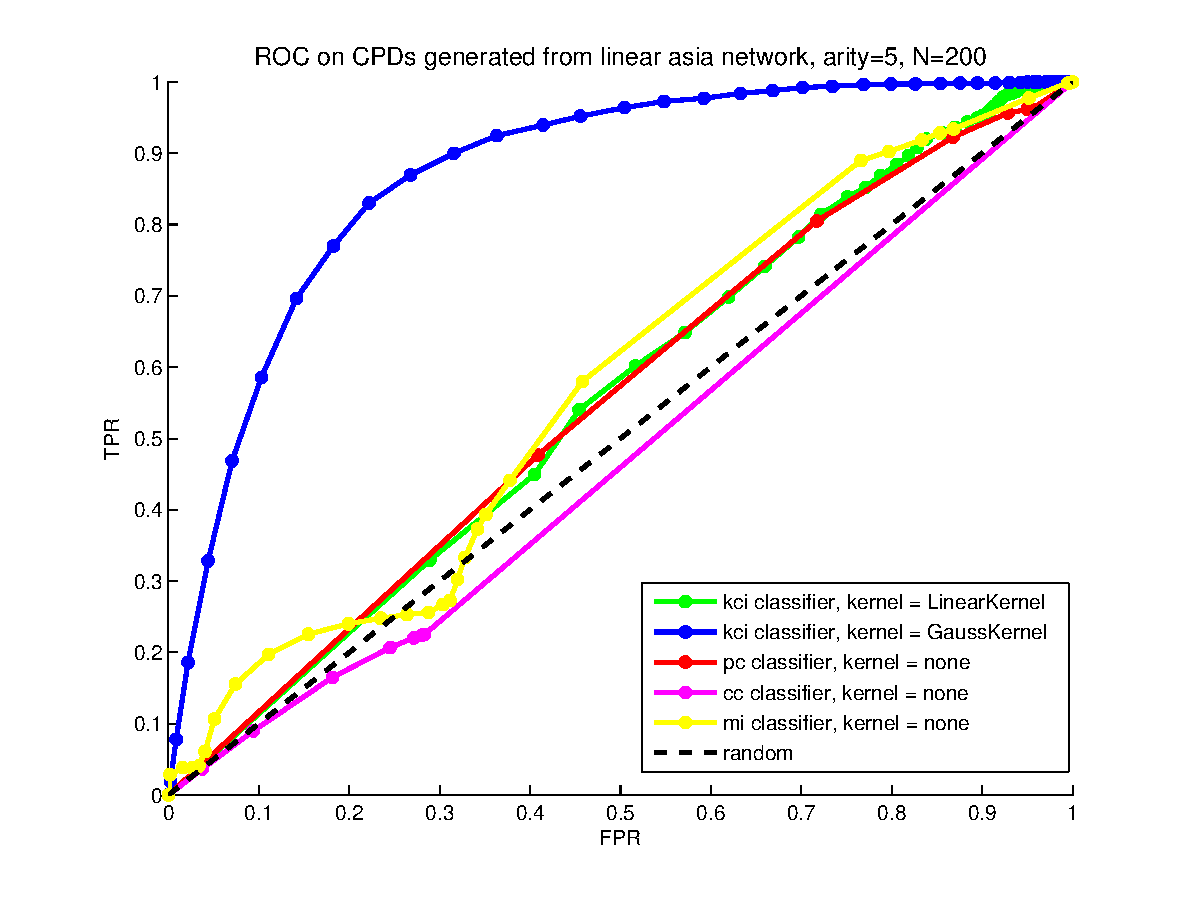
\includegraphics[width=0.45\linewidth]{img/roc_full_random_arity5.eps}
}
\subfigure{
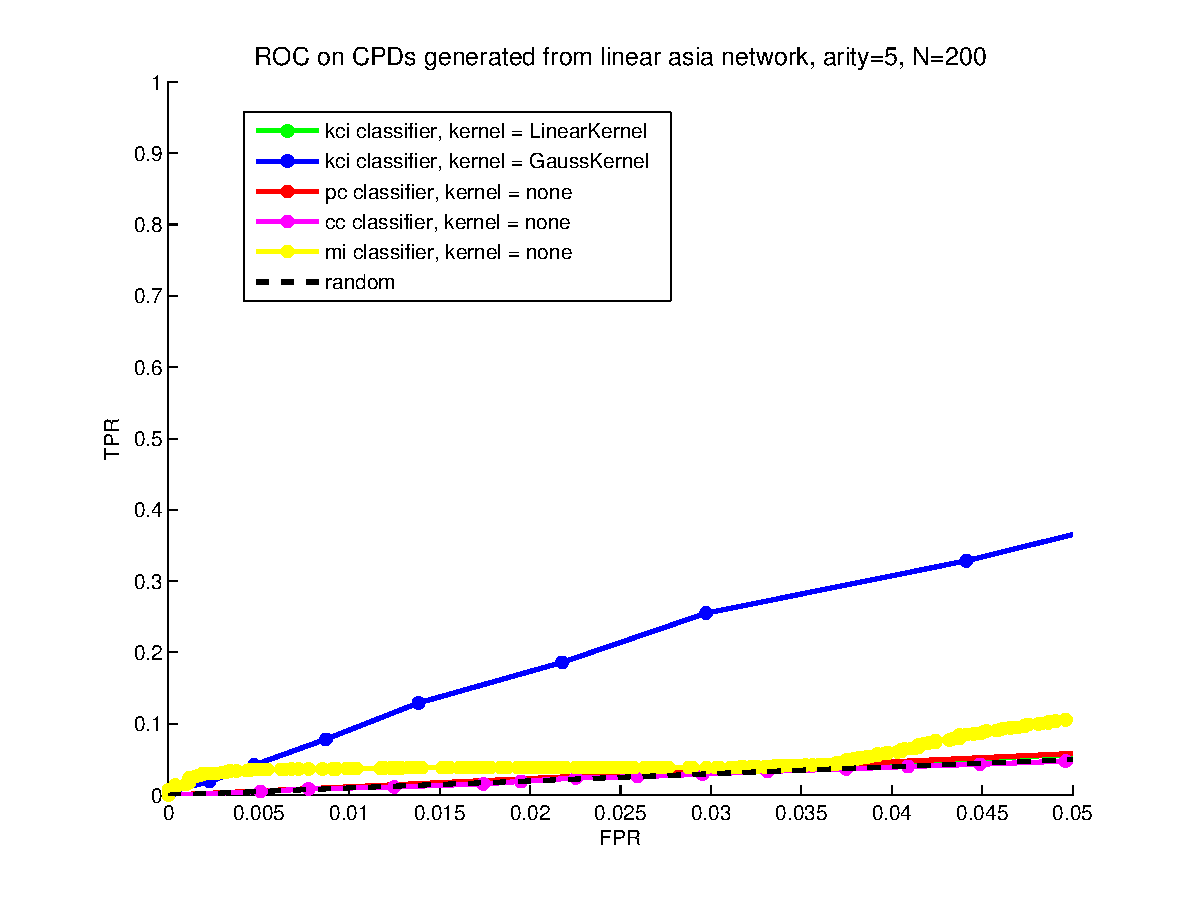
\includegraphics[width=0.45\linewidth]{img/roc_partial_random_arity5.eps}
}
\caption{Precision-recall curves for various classifiers. Plots present
results for asia network, with nodes having 5 possible classes. Local CPDs
have been chosen to express linear relation. {\bf (Left)} Entire 
precision-recall curve, {\bf (Right)} Low recall fragment of precision-recall curve.}

\end{figure}

\subsection{Classification of CPDs from Gene Expression}

\subsection{Synthetic Bayesian networks}

\subsection{Gene expression data}

\section{Discussion}

\begin{small}
%\renewcommand\bibname{References}
\bibliographystyle{abbrvnat}
%\bibliographystyle{authordate1}
%\bibliographystyle{amsnomr}
\bibliography{bibliography}
\end{small}

%\appendix
%\include{appendix}

\end{document}
